\documentclass[11pt]{article}
%Gummi|061|=)

\title{\textbf{MSWL Developers and Motivations:\\
Linus Torvalds and the Linux Kernel Project}}
\author{Sergio Arroutbi Braojos}

\date{\today}

\usepackage{hyperref}
\usepackage{amsmath}
\usepackage{mathtools}
\usepackage{varioref}
\usepackage{placeins}
\usepackage[bottom=14em]{geometry}
\usepackage{float}
\usepackage{graphicx}

\restylefloat{table}

\begin{document}

\hypersetup
{   
pdfborder={0 0 0}
}
   
\maketitle

\begin{center}
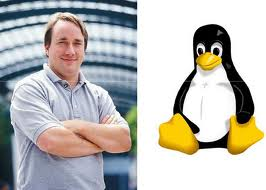
\includegraphics[width=90mm]{LinusLinux.jpeg}
\end{center}

\pagebreak

\tableofcontents
\listoffigures
\listoftables

\pagebreak

\section{Introduction}
Linus Torvalds is, surely, the most influencing person on the Open Source World. Twenty years after initiation of the Linux project by him, this open source Operating System being the main maintainer of the Linux project, this Operating System has become, surely, one of the most used and versatile Operating Systems, leader in some markets, as the Internet Servers Operating Systems or the SuperComputers Operating Systems, as well as the most important Open Source Project, at least, from an economic impact point view.\\
\\
Linus Torvalds is also creator and developer of the GIT source code control version system, the most used distributed version control system, with an increasing popularity above all on the Open Source projects enviroment. However, Torvalds turned over maintenance on 26 July 2005 to Junio Hamano, a major contributor to the project, so GIT is not a relevant aspect of the analysis of Linus Torvalds as Open Source Project Manager, compared to up to date leadership on the Linux Kernel Operating System project.

\pagebreak

\section{Biography}
Linus Torvalds [1] was born on December 28, 1969 in Helsinki, Finland. His parents were communist campus radicals in the 1960s. Other children used to tease Linus about this aspect.  His family belongs to the Swedish-speaking minority (5.5\% of Finland's population).\\ 
\\
Linus expressed how intelligent he was as at a very early age. His grandfather bought a Commodore VIC 20 when he was twelve, one of the first personal computers, and Torvalds learned to write programs, computer games among others, for it. He became obsessed with computers and programming, buying many books on the subject. When his grandfather died, he was given the computer to work on at home.\\
\\
He was described as a perfectionist and sore loser. He was very focused on computers and ignored other activities such as sports to program in solitude. He later invested in a Sinclair QL computer, which was invented by a British man named Clive Sinclair. He modified this computer extensively, especially its operating system. He programmed, among others, an assembly language and a text editor, as well as a few games.\\
\\
From 1988 to 1996, Linus studied computer science at the University of Helsinki. His academic career suffered an interruption after his first year studying, as he joined the Army, selecting the 11-month officer training program to fulfill the mandatory military service of Finland.\\
\\
When Linus Torvalds come back to the university, he invested in a better computer with a 386 processor and began learning its assembly language. He coded a number of advanced software projects, including a floppy disk driver and a software assembler.\\
\\
In 1990, he began learning Unix when the university purchased a MicroVAX system. He decided to start writing his own Unix kernel for personal computers and spent half of a year in front of the PC coding. Once he started using the C programming language, his productivity increased greatly.\\
\\
The product of his hard work became known as Linux.
Linux was released as an open source kernel, meaning that anyone could write operating systems around it without having to pay anything. It quickly became a symbol of the open source movement, with a tuxedo penguin as its mascot.\\
\\
As a result of his skills and accomplishments, Torvalds was appointed to the post of instructor at the University of Helsinki, a position which allowed him to simultaneously continue his development of Linux. One of the students, Tove Minni, a Finnish karate champion, complied by sending him an e-mail asking him out on a date. He accepted, and three years later the first of their three daughters was born.\\
\\
Over the next decade, it became more and more popular as some people, above all from computer engineering in the University, decided to abandon Microsoft Windows in favor of free operating systems that utilized the Linux kernel.\\
\\
Today, the Linux movement is still perceived as a threat to Microsoft, which currently has a tight grip on the world's personal computers. The many Linux-based operating systems include Red Hat, Knoppix, Debian, and Fedora.\\
\\
From 1997 to 2003, Linux worked for Transmeta Corporation. Later, he worked for Open Source Development Labs in Beaverton, Oregon.\\
\\
In 2004 he was named one of the world's most influential people by Time Magazine.\\
\\
He was honored with the 2012 Millennium Technology Prize, along with Shinya Yamanaka, by the Technology Academy Finland "in recognition of his creation of a new open source operating system for computers leading to the widely used Linux kernel" [3].\\
\\
He lives nowadays with his wife and three kids in Portland, and works for the Linux Foundation, the non-profit organization for promotion of the Linux Open Source Project.

\pagebreak

\section{The Linux Project}

\subsection{Project Birth} 
In early 1991, Linus Torvalds purchased an IBM-compatible personal computer with a \textbf{33MHz Intel 386 processor and a huge 4MB of memory}. Torvalds was intrigued with the hardware, as this processor greatly appealed to him because it represented a tremendous improvement over former Intel chips [3]. However, he was \textbf{disappointed with the MS-DOS operating system} that came with it. Microsoft's operating system had not advanced sufficiently to even begin to take advantage of the vastly improved capabilities of the 386 chip, and he thus strongly preferred the much more powerful and stable UNIX operating system that he had become accustomed to using on the university's computers.\\
\\
Consequently, Torvalds attempted to obtain a version of UNIX for his new computer. He could not find even a basic system for less than US\$5,000. \textbf{He also considered MINIX}, a small clone of UNIX that was created by operating systems expert Andrew Tanenbaum in the Netherlands to teach UNIX to university students. However, although much more powerful than MS-DOS and designed to run on Intel x86 processors, MINIX still had some serious disadvantages, as the facts that \textbf{not all of the source code was made public}, it lacked some of the features and performance of UNIX and there was a not-insignificant licensing fee.\\
\\
\textbf{Torvalds thus decided to create a new operating system from scratch}, based on both MINIX and UNIX. Obviously, he was not fully aware of the tremendous amount of work that would be necessary, and it is even far less likely that he could have envisioned the effects that his decision would have both on his life and on the rest of the computer science world. Because university education in Finland is free and there was little pressure to graduate within four years, Torvalds decided to take a break and devote his full attention to his project.\\
\\
On \textbf{August 25, 1991}, he announced his initial creation on the MINIX newsgroup comp.os.minix as follows:
\begin{verbatim}
Message-ID: 1991Aug25.205708.9541@klaava.helsinki.fi 
From: torvalds@klaava.helsinki.fi (Linus Benedict Torvalds) 
To: Newsgroups: comp.os.minix 
Subject: What would you like to see most in minix? 
Summary: small poll for my new operating system

Hello everybody out there using minix-

I'm doing a (free) operating system (just a hobby, won't be big and
professional like gnu) for 386 (486) AT clones. This has been brewing 
since april, and is starting to get ready. I'd like any feedback on things 
people like/dislike in minix, as my OS resembles it somewhat
(same physical layout of the file-sytem due to practical reasons)
among other things.

I've currently ported bash (1.08) an gcc (1.40), and things seem to work. 
This implies that i'll get something practical within a few months, and 
I'd like to know what features most people want.

Any suggestions are welcome, but I won't promise I'll implement them :-)

Linus Torvalds torvalds@kruuna.helsinki.fi
\end{verbatim}
On September 17 of the same year, after a period of self-imposed isolation and intense concentration, he completed a crude version (0.01) of his new operating system. Shortly thereafter, on October 5, he announced version 0.02, the first official version.\\
\\
It featured the ability to run both \textbf{the bash shell} (a program that provides the traditional, text-only user interface for Unix-like operating systems) \textbf{and the GCC} (the GNU C Compiler), two key system utilities. This now famous announcement launched the biggest collaborative project the world has ever known. It began:
\begin{verbatim}
Do you pine for the nice days of minix-1.1, when men were men and wrote their
own device drivers? 
Are you without a nice project and just dying to cut your teeth on a OS you
can try to modify for your needs? 
Are you finding it frustrating when everything works on minix? 
No more all-nighters to get a nifty program working? 
Then this post might be just for you :-)

As I mentioned a month(?) ago, I'm working on a free version of a 
minix-lookalike for AT-386 computers. It has finally reached the stage where it's even usable (though may not be depending on what you want), and I am willing to put out the sources for wider distribution. It is just version 0.02 (+1 (very small) patch already), but I've successfully run bash/gcc/gnu-make/gnu-sed/compress etc under it.

Sources for this pet project of mine can be found at nic.funet.fi 
(128.214.6.100) in the directory /pub/OS/Linux. The directory also contains 
some README-file and a couple of binaries to work under linux (bash, update 
and gcc, what more can you ask for :-). 

Full kernel source is provided, as no minix code has been used. Library 
sources are only partially free, so that cannot be distributed currently. 
The system is able to compile "as-is" and has been known to work. Heh. . . .
\end{verbatim}
Linus Torvalds had wanted to call his invention Freax("free", "freak", and "x", as an allusion to Unix). During the start of his work on the system, he stored the files under the name "Freax" for about half of a year. The files were uploaded to the FTP server (ftp.funet.fi).\\
\\
Ari Lemmke, who was one of the volunteer administrators for the FTP server at the time and  Torvald's coworker at the Helsinki University of Technology, encouraged him his source code to be uploaded to a network so it would be available for use, study, inspection and refinement by other programmers, a common practice then as it is now. Lemmke did not think that "Freax" was a name that fits. So, he re-named the project "Linux" on the server without consulting Torvalds. Torvalds consented to "Linux". He recognizes that he had already thought about that name, although he discarded the idea because thought it was too egoistical.\\
\\
In what Torvalds now admits was \textbf{one of his best decisions}, he decided to \textbf{release Linux under the GPL} (GNU General Public License) rather than under the more restrictive license that he had earlier planned. Developed by Richard Stallman, a notable programmer and a leading advocate of free software, GPL is one of the most popular of the free software licenses, above all among the ones known as "copyleft", and allows anyone to study, use, modify, extend and redistribute the software as long as they make the source code freely available for any modified versions that they create and then redistribute.\\
\\
In large part a consequence of this very liberal licensing, many programmers from around the world quickly became enthusiastic about helping Torvalds develop his still embryonic operating system. As a result, its performance began improving at a rapid rate.\\
\\
Torvalds' efforts focused on developing a kernel, which is only part of what is necessary to make a usable operating system. Fortunately, Stallman and his Free Software Foundation (FSF) had been developing a number of free programs for use in a free version of UNIX, and such programs (e.g., bash, GCC and GNU binutils) thus became major components of virtually all Linux distributions. A distribution is a complete operating system centered around a kernel and containing numerous utilities, device drivers and application programs.\\
\\
Other parts of Linux distributions came from the Berkeley UNIX Distribution (BSD), a version of UNIX that was developed at the University of California at Berkeley (UCB) and which later evolved into the highly regarded BSD operating systems. And the X Window System, which is the dominant system for managing GUIs (graphical user interfaces) on Linux and other Unix-like operating systems, came from the Massachusetts Institute of Technology (MIT).
\subsection{Project success}
Linux kernel project key for success was basically one: \textbf{Performance}. Linux kernel and Linux distributions appearing continued to improve as more and more developers, initially individual and later corporate as well, joined the project and contributed their enthusiasm, effort and programming skills. This was paralleled by a swift growth in the number of users.\\
\\
A very remarkable date for Linux Open Source project was 1994, because of different factors:
\begin{itemize}\itemsep0pt
\item{A usable ext2 filesystem, which featured a large increase in speed over its predecessor, the ext, was added to the kernel.}
\item{Linux initially weak networking capability was improved substantially.}
\item{This was also the year in which Torvalds began promoting the porting of Linux to additional processors.}
\end{itemize}
Regarding last item, Linus realized that one early complaint about Linux was that it could run only on computers with x86 (Intel-compatible) processors. Responding to this complain, Linux kernel started to be released for other processors as well. The first of the new processors was the Alpha, which was used in Digital Equipment Corporation's (DEC's) workstations. This was greatly facilitated by DEC's investment of both money and engineering talent, and it was soon followed by porting to the SPARC and MIPS processors.\\
\\
Although the arrival of his first daughter coincided with minor disruptions in the development of the Linux kernel, he was able to release version 2.0 by December 1996. This milestone version represented a major improvement in performance through its addition of support for additional processors and for symmetric multiprocessing (SMP), which lets multiple processors access and be equally close to all RAM locations.\\
\\
The use of Linux continued to grow rapidly as a result of these and numerous other advances as well as due to its spreading fame. By 1997, conservative estimates were placing worldwide Linux installations at more than three million computers. Two years later this had soared to in excess of seven million.\\
\\
Lately, and, in particular, in year 2012, Linux has considered to be of great successful due to different factors:\\
\begin{itemize}\itemsep0pt
\item{Red Hat achieving \$1billion revenue}
\item{Android increasing its position to 50 percent of American mobile market}
\item{Steam distribution platform for Linux}
\item{Adoption of Linux-based solutions from automotive industry}
\item{HP becoming a platinum Linux foundation member}
\end{itemize}
Despite the relentless successes of Linux and the great popularity of Torvalds, his activities were not entirely without controversy, even within the free software community. For example, Professor Tanenbaum, the developer of MINIX on which Linux was originally partially based, was convinced that microkernels (a minimalist type of kernel) were the wave of the future, and he expressed strong opposition to the monolithic approach of the Linux kernel in his now famous 1992 Usenet posting titled LINUX is obsolete [4].\\
\\
Also, Richard Stallman has continued to insist that Linux's name is inappropriate and that the operating system should instead be renamed GNU/Linux because Stallman's numerous GNU utilities are used together with the Linux kernel, as stated on the Film "Revolution OS" [5].

\subsection{Project Governance}
The Linux Kernel project is a typical case of what is considered to be a project under a Benevolent Dictator For Live (BFDL) [6], who applies to the project a strong, centralized leadership. Linus Torvalds as the founder and BDFL sets the agenda and also appoints strong lieutenants, so most issues do not require his attention until they're ready for commit. Anybody can submit a patch to the mailing list, but getting it accepted is very much a matter of working with the chain of command.\\
\\
In an interview [8], Torvalds recognizes no hierarchy exist on the project. The kernel is more based on a trusted relationship network. He recognizes having around 50 trusted people, and suggest that people also have trusted people as well for their particular stuff. 
\subsection{People around Linus}
Linux kernel is a project with more than 17 million source code lines [7]. Taking into account this number, it is an obvious thing that the project is not managed completely by Linus Torvalds. Difficult to find a hierarchy graph about the project governance, there is somehow a kind of delegation in two manners:
\begin{enumerate}
\item{\textbf{The maintainer list}}. Linux kernel project contains a list of maintainers for patches to be sent. By November 2013, there is a list of 900 maintainers, handling the different drivers, CPU architectures, virtualization stuff, network layers, etc.
\item{\textbf{Top Reviewers}}. As showed in the Linux Foundation Report: "Who writes Linux 2013", Senior Kernel Developers are more dedicated to review code from contributors. On this report, the list of "10 Top Reviewers", as described in Table~\ref{tab:topreviewers}.
\begin{table}[H]
  \begin{center}
    \begin{tabular}{ | l | l | l | }
    \hline
    Name & Signoffs & Percent \\
    \hline
    Greg Kroah-Hartman    & 9,965 & 12.5\%\\
    David S. Miller       & 6,133 &  7.7\%\\ 
    Mauro Carvalho Chehab & 3,847 &  4.8\%\\
    John W. Linville      & 3,541 &  4.4\%\\
    Andrew Morton         & 3,403 &  4.3\%\\
    Mark Brown            & 2,479 &  3.1\%\\
    James Bottomley       & 1,246 &  1.6\%\\
    Daniel Vetter         & 1,192 &  1.5\%\\
    Ingo Molnar           & 1.012 &  1.3\%\\
    Samuel Ortiz          &   984 &  1.2\%\\
    \hline
    \end{tabular}
    \caption{Top Reviewers}
    \label{tab:topreviewers}
  \end{center}
\end{table}

\item{\textbf{Top Commiters List}}. Previous described report also shows the most important contributors to the Linux Kernel Project. The list is described in Table~\ref{tab:topcommitters}.
\begin{table}[H]
  \begin{center}
    \begin{tabular}{ | l | l | l | }
    \hline
    Name & Changes & Percentage\\
    \hline
    Al Viro                    & 4,124 & 1.2\%\\
    David S. Miller            & 3,690 & 1.0\%\\
    Takashi Iwai               & 3,387 & 1.0\%\\
    Mark Brown                 & 3,199 & 0.9\%\\
    Tejun Heo                  & 2,888 & 0.8\%\\
    Johannes Berg              & 2,841 & 0.8\%\\
    Mauro Carvalho Chehab      & 2,718 & 0.8\%\\
    Russell King               & 2,526 & 0.7\%\\
    Greg Kroah-Hartman         & 2,502 & 0.7\%\\
    Thomas Gleixner            & 2,423 & 0.7\%\\
    H Hartley Sweeten          & 2,415 & 0.7\%\\
    Ingo Molnar                & 2,376 & 0.7\%\\
    Paul Mundt                 & 2,268 & 0.6\%\\
    Bartlomiej Zolnierkiewicz  & 2,076 & 0.6\%\\
    Hans Verkuil               & 2,074 & 0.6\%\\
    Alan Cox                   & 1,962 & 0.6\%\\
    Adrian Bunk                & 1,919 & 0.5\%\\
    Christoph Hellwig          & 1,877 & 0.5\%\\
    Ralf Baechle               & 1,840 & 0.5\%\\
    Joe Perches                & 1,839 & 0.5\%\\
    \hline
    \end{tabular}
    \caption{Top Committers}
    \label{tab:topcommitters}
  \end{center}
\end{table}

\item{\textbf{Releases Maintenance}}
From Long-term based releases, most important responsibles are defined in Table~\ref{tab:releasemaintainers}:
\begin{table}[H]
  \begin{center}
    \hspace*{-2cm}\begin{tabular}{ | l | l | l | }
    \hline
    Release & Maintainer & Release Description\\
    \hline
    \hline
    2.6.32 & Willy Tarreau & 3rd long-term stable release from December 2009 to mid 2014\\
    & & Used in Debian 6 Squeeze\\
    \hline
    2.6.34	& Paul Gortmaker & 5th long-term stable release from January 2011 to mid 2013\\
    \hline
    3.2	5  & Ben Hutchings	& 8th long-term stable release from March 2012 to 2016\\
    & & Used in Ubuntu 12.04 LTS, Debian 7 Wheezy and Slackware 14.0\\
    \hline
    3.4	   & Greg Kroah-Hartman & 9th long-term stable release from May 2012 to October 2014\\
    \hline
    3.10   & Greg Kroah-Hartman & 10th long-term stable release from August 2013 to September 2015\\
    \hline
    3.11   & Greg Kroah-Hartman	& Stable version.\\
    \hline
    3.12   & Linus Torvalds	& Latest stable version.\\
    \hline
    3.13   & Linus Torvalds	& Latest preview version.\\
    \hline
    \end{tabular}
    \caption{3.0 Kernel Release Maintainers}
    \label{tab:releasemaintainers}
  \end{center}
\end{table}
\end{enumerate}

Previous lists show important people who are really very important roles for the Linux Kernel project:
\begin{itemize}\itemsep0pt
\item{\textbf{Greg Kroah-Hartman}}: Definitely, the second most important person for the kernel projects according to the statistics above. Top reviewer, several branch maintainer and in the "Top 10" commiter group.
\item{\textbf{David S. Miller}}: Being second top commiter and the second top reviewer as well, David S. Miller is definitely one of the nowadays top important people in the project.
\end{itemize}
There have been also important contributors to the Linux Kernel who have quit from the project.
\begin{itemize}\itemsep0pt
\item{\textbf{Alan Cox}}: Born in 1968, Cox was a very active Linux kernel developer in the past. Considered the number 2 in the Linux world for the initial period of Linux history (1991-2002). Before becoming a maintainer of the 2.2 production version of the kernel, he also was the maintainer of network stack, one of the most critical parts of the Linux kernel [10]. He quit from Linux project on January 2013, due to family issues[11]:
\begin{verbatim}
"I’m leaving the Linux world and Intel for a bit for family reasons,” 
he wrote. “I’m aware that ‘family reasons’ is usually management speak for 
‘I think the boss is an asshole’ but I’d like to assure everyone that while
I frequently think Linus is an asshole (and therefore very good as 
kernel dictator). I am departing quite genuinely for family reasons and not
because I've fallen out with Linus or Intel or anyone else. 
Far from it I've had great fun working there."
\end{verbatim}
\end{itemize}

\subsection{Project Release System}
On version 1 of the kernel, releases happened frequently. Later, for version 2 of the kernel, release dates started growing. 2.2 Kernel release version happened in January 1999, after two years and a half from kernel 2.0. Kernel 2.4 release happened in January 2001, after two years of 2.2 release. Kernel 2.6 release happened on December 2003, after almost three years of 2.4 release. Starting in 2004, the release process changed, and new kernels started coming out on a regular schedule every 2–3 months, numbered 2.6.0, 2.6.1, up through 2.6.39. On 21 July 2011 Linus Torvalds announced the release of Linux 3.0. When releasing this kernel version, he asserted:
\begin{verbatim}
"Gone are the 2.6.<bignum> days".
\end{verbatim}
The big number version change  is not about major technological changes, but rather marks the kernel's 20th anniversary. So, from that date, the project release dates follow a "Release Often, Release Early" basis associated to the second number (rather than third) of the second release version. Table ~\ref{tab:releasedates} shows kernel 3.0 branch release dates and days of development
\begin{table}[H]
  \begin{center}
    \begin{tabular}{ | l | l | l | }
    \hline
    Kernel Version & Release Date & Days of Development\\
    \hline
    3.0  & 2011-07-21 & 64\\
    3.1  & 2011-10-24 & 95\\
    3.2  & 2011-12-31 & 68\\
    3.3  & 2012-03-18 & 74\\
    3.4  & 2012-05-20 & 63\\
    3.5  & 2012-07-21 & 62\\
    3.6  & 2012-09-30 & 71\\
    3.7  & 2012-12-10 & 71\\
    3.8  & 2013-02-18 & 70\\
    3.9  & 2013-04-28 & 69\\
    3.10 & 2013-06-30 & 63\\
    \hline
    \end{tabular}
    \caption{3.0 Kernel Release Dates}
    \label{tab:releasedates}
  \end{center}
\end{table}

\pagebreak

\section{Linus Torvalds: The (not so?) Benevolent Dictator}
\subsection{Current role}
Linus Torvalds is the Founder of the Linux Kernel project, and has performed also the leader role for more than 20 years. Only this data gives an idea of his persevering nature.\\
Not being dedicated to committing much code any more (he is not in the top 20 commiters neither the top 10 reviewers in the project), Torvalds performs perfectly the role of Leader by:
\begin{itemize}\itemsep0pt
\item{Getting other developers’ patches into the kernel}
\item{Driving the project maintainer list}
\item{Routing accepted patches toward the mainline}
\item{Spreading the project by giving talks and interviews}
\item{Driving latest branches, and performing branch management}
\item{Performing the role of the benevolent dictator, by making the final decissions on the top issues where no consensous is achieved}
\end{itemize}
Linus Torvalds importance for Linux project success has been enough evidence given through the years. The community, among other facts, recognizes specially that Torvalds designed in a very short period of time the core of an Operating System that proved to be modular, simple (as simplicity can be applied to an Operating System), and, above all, having a great performance in terms of both robustness and efficiency.\\
But the community recognizes as well that the simplicity, modularity and licensing schema helped on spreading the project quickly and easily through years, for both contributors and final users as well.\\
The project itself, along the years, has turned to be the market share leader of different important markets, such as Internet Servers, Supercomputers or Mobile Devices (as part of the Android project).

\subsection{Skills}
So far, a description of Linus Torvalds and the Linux Project has been performed. However, an analysis of the main characteristics of the Benevolent Dictator can help on determining both the project success and the community recoginizing to him. Among the different Torvald's characteristics, next must be highlighted:
\begin{itemize}
\item{\textbf{Technical engineering excellence.}}
Linux Kernel Project excellence itself allows to demonstrate Torvald's engineering excelence. Having designed it when he was just 22 years old, the simplicity of the kernel architecture and its modularity, together with the great robusteness, allow to assert that Torvalds was at a very early age, an excellent engineer.\\
Besides this, his other great work, GIT, has been proven to be a magnificient designed control version system. Indeed, the control version system has supposed a revolution on this market, and is being acquired in a lot of Open Source Projects as well as Software companies.
\item{\textbf{Resolvent}.} Torvalds has more than once proven that is a resolvent computer engineer and leader as well. When problems appear, Linus Torvalds appears under the guise of resolution.\\
This is the case of GIT birth. When the problem appeared, by the copyright holder of BitKeeper, Larry McVoy, withdrawing free use of the product after he claimed that reverse-engineering of the BitKeeper protocols had been performed, Torvalds and others grasp the nettle by designing a BitKeeper inspired control version named GIT.
\item{\textbf{Constant}.} Being for more than 20 years acting as leader of the most important Open Source project gives an idea of how constant Torvalds is.\\
Far from appearing tired, it seems that, as time goes by, Linus Torvalds continues to be as enthusiastic and commited with the project as never.
\item{\textbf{Analytical}.} Far from his technical excellence as developer, Torvalds is even more recognized for his analytical and designing capacities.\\
Behind his decissions, Torvalds has proved to have an excellent nature to understand the issues and accomplish the solutions. Core Linux kernel designing is a good example of how simplicity and modularity can help on building an Operating System to boost performance.\\
GIT is a good example as well, as it shows how some design decissions have helped this distributed control version system to be the prefered one for certain projects. 
\item{\textbf{Self-confident (sometimes to rudeness)}.}
When participating on a discussion, Torvalds always show determination and self reliance. He does not hesitate on arguing an eminence as Andrew S. Tanembaum when he has take up the cudgels of his project [12]: 
\begin{verbatim}
You use this as an excuse for the limitations of minix? Sorry, but you
loose: I've got more excuses than you have, and linux still beats the
pants of minix in almost all areas.  Not to mention the fact that most
of the good code for PC minix seems to have been written by Bruce Evans.
\end{verbatim}
Despite the fact that Torvalds has several times being pointed as a flame initiator, not to say the various times that he has replied in order to defense himself from others accusations [13]. However, the good news are that he seems to be conscious of this[14]:
\begin{verbatim}
"Sometimes being polite drives to misunderstanding on the Internet"
\end{verbatim}
\item{\textbf{Charismatic}.} Many of his strenghtness, some of them previously described, and aceptation of his weakness (rudeness above all), make him a charismatic, well recognized, awarded and charismatic person, the most important in the Open Source history ever.\\
Together with his acid sense of humour, make Linus one of the most interesting people to listen in conferences and interviews, not only in the Source Project world.
\item{\textbf{Practical and Pragmatic}.}
Regarding the Open Source Universe, the characteristic that best fits into Torvalds character is pragmatism, above all if compared to the other most important person in the Open Source Universe, Richard M. Stallman, who represents the most idealistic view. Next sectio shows this contrast deeper, but, in order to show how practical Torvalds can be, one of his favourite sentences can be included as example:
\begin{verbatim}
"Show me the code". 
\end{verbatim}
He has also asserted [8]:
\begin{verbatim}
It was Edison who said ‘1\% inspiration, 99\% perspiration’.
That may have been true a hundred years ago. These days it's ‘0.01\%
inspiration, 99.99\% perspiration’, and the inspiration is the easy part. 
As a project manager, I have never had trouble finding people with crazy 
ideas. I have trouble finding people who can execute.
\end{verbatim}
\end{itemize}
\subsection{The pragmatic view}
Talking about Open Source projects, communities, visions and missions, the same issue is brought foreground. Inside Open Source Software/Free Software two currents are found.\\
\\
On the one hand, the idealistic current, with Free Software Foundation as representative association and Richard M. Stallman as ambassador.
On the other hand, the pragmatic approach, with Open Source Initiative as representative association, and Bruce Perens and Eric Raymond as ideologues.\\
\\
It is not the aim of this document to enter details on the differences between both currents. Indeed, understanding of Open Source/Free Software is very similar. But some differences exist. In the end, a very lax summary approach around currents differences could be:
\begin{itemize}\itemsep0pt
\item{The Open Source Initiative definition of Open Source Software is smoothly less restrictive compared to the Free Software Foundation definition of Free Software.}
\item{The pragmatic current focuses on \textbf{Open Source as a tool to produce and improve software} versus the idea of the Free Software Foundation, which focuses on Free Software as a tool for users freedom obatining when using computer and other devices.}
\end{itemize}
Where does Torvalds stand inside this two currents? Licensing method selected by Torvalds for Linux Kernel project was GPLv2, which is in turn the FSF defined license to ensure spreading software by obligation of re-distribution of the changes performed on software under this license, on what is known as "copyleft". Indeed, Torvalds has ensured [14]:
\begin{verbatim}
"I am very happy with GPL...
In the very beginning, I made my own licensing version, but was wrong 
in some concepts, such as not charging any money for Linux. That would 
have become a problem if change to GPL had not been performed...
I give this out, because I like doing it, but I want people doing changes 
and improvement to come back. License clearly works very well."
\end{verbatim}
However, \textbf{Torvald's self characteristics drive him to the pragmatic side}, basically due to his skills and his practical driven nature. The Benevolent Dictators prefers:
\begin{enumerate}\itemsep0pt
\item{\textbf{Code rather than ideas}}
\item{\textbf{Things done rather than ideas proposed}}
\item{\textbf{Day to day results rather than innovation}}
\end{enumerate}
The pragmatic side in general, and Eric Raymond in particular, as stated in the Catheedral and the Bazaar [15], has always demonstrated admiration for the Benevolent Dictator, in what is a declaration of intent in recognition on how \textbf{the pragmatic view, once implemented, can drive to successful projects, with the Linux Kernel project as the most representative success story}.
\subsection{Leadership: How Torvalds commands Linux}
Volumes have been written about Linus Torvalds and the role he plays on the Linux kernel project leadership. There can be no doubt about this asertion: \textbf{In a huge Open Source project as the Linux Kernel Project, with thousands of people and dozens of companies involved, it must not be an easy thing to drive all the opinions and interests to a common point}.\\
\\
When asked, in a conference, for those things that bother him, Torvalds replied [14]:
\begin{verbatim}
The technical problems are not a big deal.
The two areas where we have issues are:
1 - Documentation from manufacturers. ... Hopefully this problem is going away.
2 - The big problem. It is hard to manage a big project with thousands of people 
and tens or hundreds of companies contributing which in turn have completely 
different point of views of where to go.
...
If I loose sleep about something, it is always about politics and is always 
about people.
\end{verbatim}
\textbf{With this basic idea in mind, how is Linux Kernel project managed?}\\
\\
Indeed, it is driven as any other Open Source project. Based on a "do-ocracy" basis, the Linux Kernel project is a clear example of a Bazaar based project management. Associated to this idea, Torvalds recognizes that, in an Open Source project, normal hierarchies do not apply[9]:
\begin{verbatim}
It is not a hierarchy. It works rather than a network, based on a matter 
of trust. It is not the traditional graph with me on the top, and 5 lieutenants
below, and each of them with several people below, it does not work like that,
with me as a traditional CEO.
\end{verbatim}
However, Torvalds also recognizes that they have no organization issues, although there is an organization [9]:
\begin{verbatim}
We don't have organization problems because we don't have an organization.
We do have one, but it is more in the conexion between people than something 
external.
\end{verbatim}
Besides this, the Benevolent Dictator asserts that someone cannot trust in all the people, or even in many people, as happens in real life. Regarding this fact, Torvalds asserts [9]:
\begin{verbatim}
Although there are thousands of people involved in arelease, I have few people 
I trust in. Around fifty. I cannot trust in everybody, in a similar way as I 
don't have hundred of friends. I can have them on Facebook, but they are not
people I trust in.
\end{verbatim}
So, from management perspective, the project works as a trusted network, where there are some nodes which are, somehow, more centralized, and contain more links to others[9.b]:
\begin{verbatim}
There are several levels of connectedness. It is a network, but, some people 
are better networked than others, and are more central in the network.
\end{verbatim}
Meanwhile, regarding his project leadership and how he has kept as the project leader for a long time, he recognizes that his abilities, besides the technical thing, have to do with the "meritocracy" obtained along the time [9.b]:
\begin{verbatim}
The reason why I am an effective project maitainer is not because I am 
technically superior to everybody else in the world. I like to think I am, 
but that is not the fundamental thing. The main reason is just that people 
trust me, not to always make the right decission, but they know how I work. 
They trust me the way somebody trusts on you after knowing you
for more than 20 years.
\end{verbatim}
Regarding the more personal relationship thing, Torvalds has been sometimes blamed to be excesively rudeness [13]. The Benevolent Overlord looses his "benevolent" nature due to dissenting voices like this, but defends himself with the argument that, on Internet, for others to understand the message, this one has to be crystal clear [14]:
\begin{verbatim}
In the Internet, we have a lot of people disappointed because their work 
was not used. Sometimes I get really frustrated, and flame people, and I 
call them dirty names.
...
I think we are solving the problem, as in the past flames were even worst, 
with discussions lasting for months.
...
When you develop the way we develop, you have to be able to let people know 
what you are thinking. If you are shuttle in the Internet, nobody gets it.
\end{verbatim}
So, as a conclussion to the way Linus Torvalds manages the kernel, with the good things and the bad things, it must be highlighted that, after more than 20 years, no forks have been performed successfully, meaning that he is doing very well his job.\\
\\Flames have to be considered a part of the deal, as they are in any other project, where tensions and discussions are the normal thing on the project execution, always while it is a controlled issue that does not increase along the time. Even better when the Benevolent Dictator recognizes that the project in general and himself in particular are improving this issue as project goes by.

\pagebreak

\section{Conclussions}
Linux kernel project is, definetely, the most important Open Source project ever. Together with some GNU applications, such as the bash shell and the GCC compiler, Linux has helped on providing the users an Open Source Operating System alternative to Microsoft Windows and Apple Mac OS. It is an Open Source alternative, costless, that every human being should, if not massively use, at least test.\\
\\
Its proven effectiveness, performance, modularity and maturity has taken this Operating System kernel to be massively used, turning it to be market share leader on different important computing markets, such as Internet Servers or Super-Computers. Besides this, the spread of the Android Operating System, relying on Linux kernel, has performed a further step for the project, into mobile handhelds.\\
\\
And, as the founder and most representative role of the movie, its founder and project leader during the last 22 years appears. During this time, with its strenghts and weakness, Linus Torvalds has demonstrated to be a great computer programmer and better designer and architecture, mainly because of the creation and leadership in the Linux kernel, but also with the design and implementation of GIT, where, not being the main maintainer neither being involved any more, the Benevolent Overlord played an important role together with other people in what seems to be the top preferred versions in the distributed Source Code Management systems.\\
\\
Beyond this, Torvalds is also recognized as a magnificient project leader, even from people who has quit from the project and has been involved, somehow, in acid discussions with him, as Alan Cox has [11].\\
\\
Due to all these reasons, Torvalds can be definetely named as the most influencing person in Open Source. And the very good news are that it seems he is definetely keep on going and still a lot to offer to the Open Source community.

\pagebreak

\section{References}
[1] \url{http://www.freeinfosociety.com/article.php?id=99}
\newline
[2] \url{http://www.technologyacademy.fi/blog/2012/04/19/laureates/}
\newline
[3] \url{http://www.linfo.org/linus.html}
\newline
[4] \url{http://www.linfo.org/linuxobsolete.html}
\newline
[5] \url{http://www.revolution-os.com/}
\newline
[6] \url{http://randyfay.com/content/how-do-open-source-communities-govern-themselves}
\newline
[7] \url{http://go.linuxfoundation.org/l/6342/-pub-who-writes-linux-2013-pdf/t5dzm}
\newline
[8] \url{https://www.simple-talk.com/opinion/geek-of-the-week/linus-torvalds,-geek-of-the-week/}
\newline
[9.a] \url{http://www.youtube.com/watch?v=fa01V0u_ybg}
\newline
[9.b] \url{http://www.youtube.com/watch?v=QHJfTja0VOs}
\newline
[10] \url{http://www.softpanorama.org/People/Cox/index.shtml}
\newline
[11] \url{http://www.wired.com/wiredenterprise/2013/01/alan-cox/}
\newline
[12] \url{https://groups.google.com/forum/?fromgroups=#!topic/comp.os.minix/wlhw16QWltI}
\newline
[13] \url{http://www.attendly.com/linux-founder-linus-torvalds-delivers-a-smackdown-like-no-other/}
\newline
[14] \url{https://www.youtube.com/watch?v=__fALdvvcM0}
\newline
[15] \url{http://www.catb.org/esr/writings/homesteading/cathedral-bazaar/}
\newline
[16] \url{http://firstmonday.org/ojs/index.php/fm/rt/printerFriendly/1481/1396}
\end{document}
